%! TEX root = ../main.tex
\documentclass[main]{subfiles}

\begin{document}
\silentchapter{\texorpdfstring
{(分子の次数)$\geqq$(分母の次数)$\rightarrow$整式の剰余で字数下げ}
{}}

\begin{mondai}{10}{今週の積分}{***}
    \begin{align*}
        \int_{0}^{2} \frac{3x^3 + 12x + 1}{x^2 + 4} dx
    \end{align*}
\end{mondai}

\approachitem{分数関数では,分子の次数を分母の次数より小さくするのが鉄則.}

\solutionhead
\hfill
以下に計算手順を示す.
\hfill\

\begin{align*}
\int_{0}^{2} \frac{3x^3 + 12x + 1}{x^2 + 4} dx &= \int_{0}^{2} \frac{3x(x^2+4)+1}{x^2+4} dx \\
&= 3\int_{0}^{2} x \, dx + \int_{0}^{2} \frac{1}{x^2+4} dx
\end{align*}

\Itembox{
    x = 2 \tan\theta \qquad 
    \begin{tabular}{c|ccc}
        $x$ & $0$ & $\rightarrow$ & $2$ \\ \hline
        $\theta$ & $0$ & $\rightarrow$ & $\frac{\pi}{4}$ \\
    \end{tabular} \qquad
    dx = \frac{2}{\cos^2\theta} d\theta
}

\begin{align*}
&= 3 \left[ \frac{x^2}{2} \right]_{0}^{2} + \int_{0}^{\frac{\pi}{4}} \frac{1}{4(\tan^2\theta+1)} \cdot \frac{2}{\cos^2\theta} d\theta \\
&= 6 + \frac{1}{2} \int_{0}^{\frac{\pi}{4}} d\theta \\
&= 6 + \frac{\pi}{8}
\end{align*}

\begin{figure}[H]
\centering
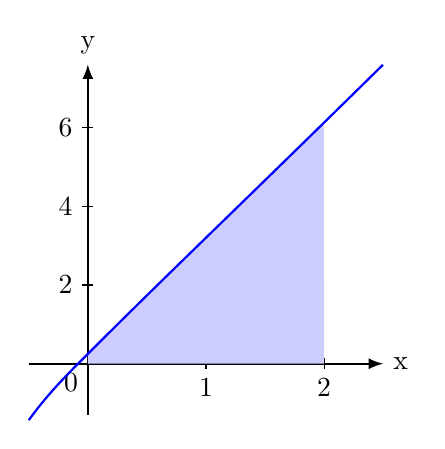
\begin{tikzpicture}[x=1.5cm, y=0.5cm]
% --- 座標軸の描画 ---
\draw[-latex, thick] (-0.5,0) -- (2.5,0) node [right] {x};
\draw[-latex, thick] (0,-1.3) -- (0,7.6) node [above] {y};

    % --- 目盛りの描画 ---
    \foreach \x in {1,2} {
        \draw (\x,2pt) -- (\x,-2pt) node [below] {$\x$};
    }
    \foreach \y in {2,4,6} {
        \draw (2pt,\y) -- (-2pt,\y) node [left] {$\y$};
    }
    \node [below left] at (0,0) {$0$};

    % ★★★ グラフとx軸、x=0、x=2で囲まれた領域を塗りつぶす ★★★
    \fill [blue!20] (0,0) -- plot [domain=0:2, samples=100, variable=\x] (\x, {(3*\x^3 + 12*\x + 1)/(\x^2 + 4)}) -- (2,0) -- cycle;

    % --- 関数のプロット ---
    \draw [domain=-0.5:2.5, samples=100, smooth, variable=\x, blue, thick] plot ({\x}, {(3*\x^3 + 12*\x + 1)/(\x^2 + 4)});

\end{tikzpicture}
\caption{$y=\frac{3x^3 + 12x + 1}{x^2 + 4}$ のグラフと $0 \le x \le 2$ の領域}
\label{fig:rational_function_filled_tikz}
\end{figure}

\begin{focusbox}
\centering
\textbf{(分子の次数)$\geqq$(分母の次数)$\rightarrow$整式の剰余で字数下げ}
\end{focusbox}

\end{document}